\chapter{3D Tree Modeling Using Motion Capture}
\label{chap:treeparticles}

\noindent
Jie Long and Michael Jones. 3D Tree Modeling using Motion Capture. \emph{IEEE The Fourth International Symposium on Plant Growth Modeling, Simulation, Visualization and Application (PMA '12)}, to appear.

\begin{abstract}
Recovering tree shape from motion capture data is a first step toward efficient and accurate animation of trees in wind using motion capture data. Existing algorithms for generating models of tree branching structures for image synthesis in computer graphics are not adapted to the unique data set provided by motion capture. We present a method for tree shape reconstruction using particle flow on input data obtained from a passive optical motion capture system. Initial branch tip positions are estimated from averaged and smoothed motion capture data. Branch tips, as particles, are also generated within bounding space defined by a stack of bounding boxes or a convex hull. The particle flow, starting at branch tips within the bounding volume under forces, creates tree branches. The resulting shapes are realistic and similar to the original tree crown shape. Several tunable parameters provide control over branch shape and arrangement.
\end{abstract}

\section{Introduction}

Reconstruction of tree shape from motion capture data is an important step in replaying motion capture of trees under external forces, such as natural wind. Motion capture provides a fast and easy way to collect the locations over time of retroreflective marker locations placed on an object. In this paper, we address the problem of creating 3D tree shape from motion capture data. We also discuss best practices for collecting motion data from a tree. This research focuses on reconstructing static 3D tree shape with branching skeletons from data collected by a motion capture system.

\begin{figure*}[!t]
\centering
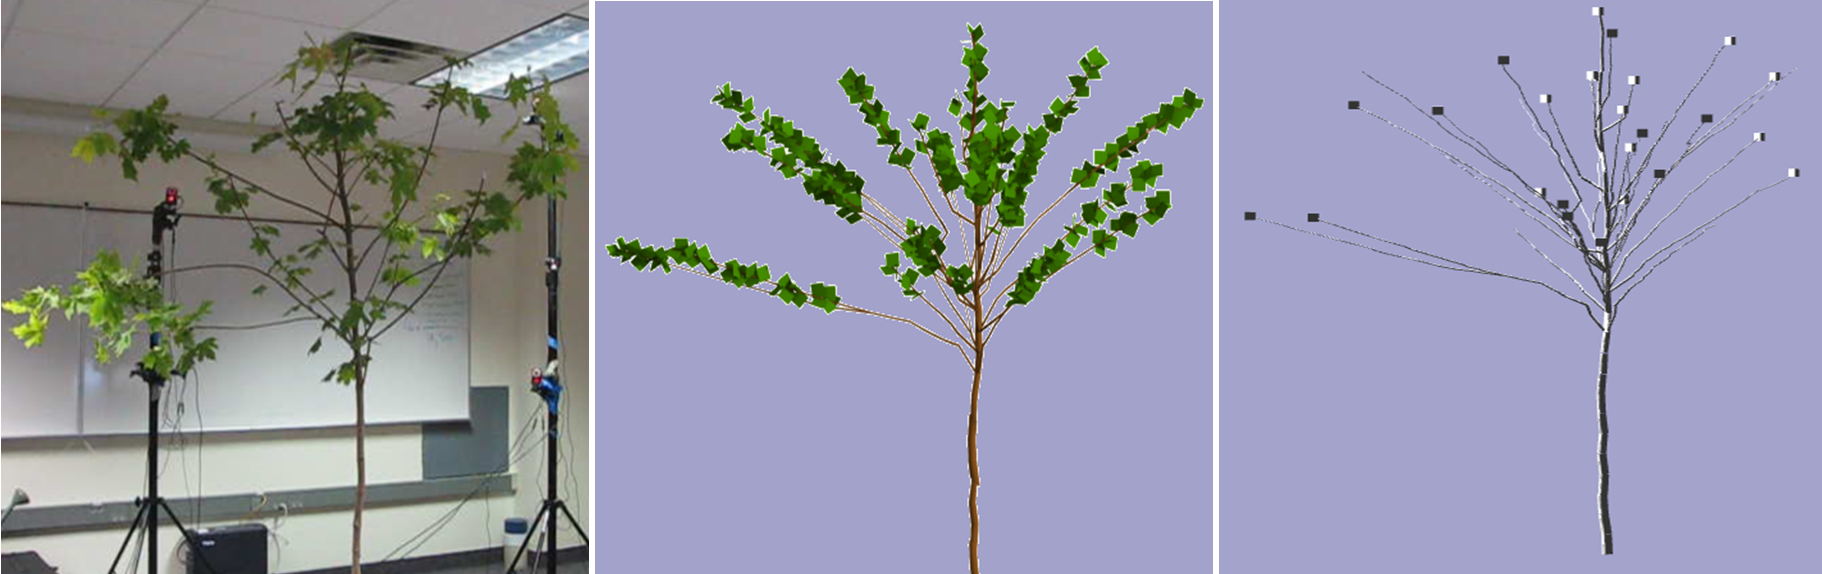
\includegraphics[scale=0.27]{Maple}
\caption{Maple model.}
\label{fig:treemodelssubfig2}
\end{figure*}

\begin{figure*}[!t]
\centering
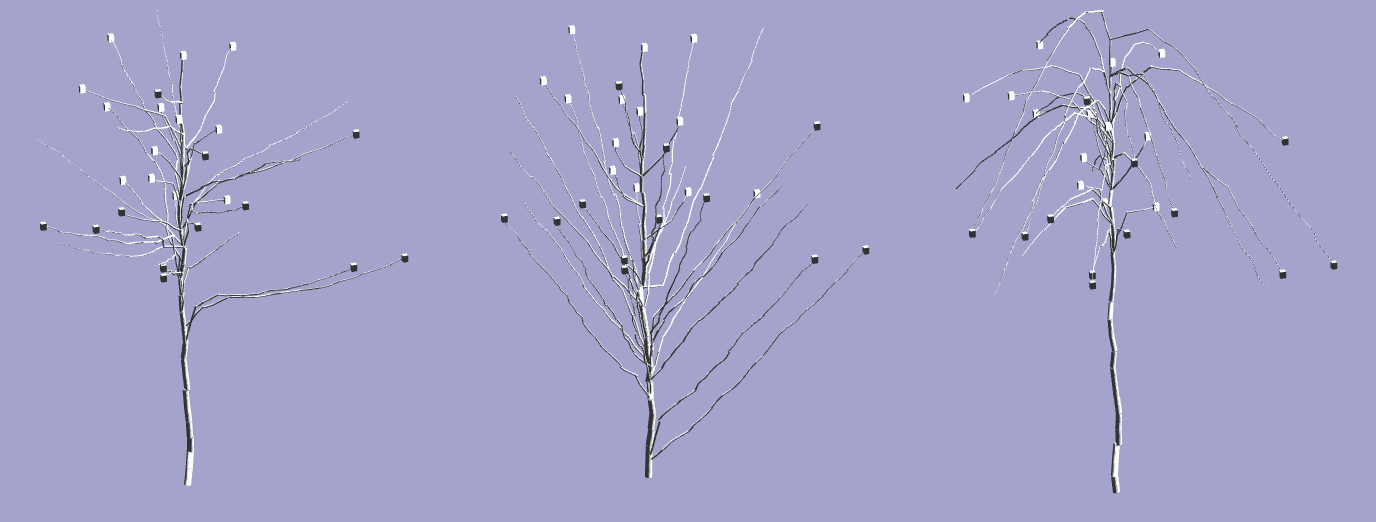
\includegraphics[scale=0.36]{varTree}
\caption{Various tree shapes generated from the same set of motion capture data. }
\label{fig:varTree}
\end{figure*}

Solutions to the motion capture problem for trees can be applied to problems in visual effects and the study of tree motion. Motion capture is a potential solution because motion capture data includes effects that are difficult to model in simulation, such as variable branch stiffness, non-uniform variation in size, and emergent effects due to leaf deformation.

Tree shape modeling has long been studied in computer graphics.  Past methods include particle systems \cite{Reeves83particlesystems,Runions07,palubicki:siggraph09,neubert:acmtg07}, L-systems \cite{lindenmayer68,Lintermann1999,Prusinkiewicz:2001}, parametric models \cite{Weber1995}, photographs \cite{RecheMartinez2004,neubert:acmtg07,Tan:2007:ITM}, and videos \cite{Li:2011:MGM,Diener:2006}. Most of these methods result in satisfying tree shapes but do not leverage the 3D positions of motion capture markers, which are recorded as part of a motion capture session but require a different set of inputs. Image- or video-based approaches convert a set of 2D input images into 3D tree models by filling in the missing dimension.  Motion capture systems can record tree shape in 3D with high precision (using similar techniques for converting a set of 2D images to a 3D model). Prior work in reconstructing tree shape from motion capture data using either exact measurements or markers placed within the crown does not scale and does not apply when leaves occlude the branching structure.

We reconstruct 3D tree shape using particle flow with motion capture data as input. Passive optical motion capture\footnote[1]{http://www.naturalpoint.com/optitrack/} records locations of reflective markers in the capture arena. We place markers only at branch tips on the edge of the tree crown. Approximately 30 markers cover the crown shape of a medium-sized tree. We do not put markers on each branch tip because passive optical motion capture systems cannot reliably track more than 70 markers. A particle flow algorithm generates branching structures starting at the recorded tip positions. Additional starting points are defined within the estimated volume of the tree crown using a vertical stack of bounding boxes or a convex hull. The bounding space approximates the tree crown and bounds particle flow and creation. The step length of a particle's flow varies with the distance to the nearest trunk point. The direction of particle motion is a combination of three forces: gravity, shape-format, and wind. The shape-format guides the particles to preserve the original tree shape. The dominant wind direction is recorded during the motion capture process. We also introduce two vectors with one pointing to the nearest trunk point and the other pointing to a constant predefined attractor point. These vectors are factors for the direction and magnitude of the forces.

In this paper, we propose a new particle flow method for reconstructing tree shape from only motion capture data. Our primary contributions are 
\begin{itemize}
	\item {a simplified particle flow algorithm for constructing tree shapes from a sparse set of branch tip positions as collected as part of motion capture and}
	\item {a method for deploying passive optical motion capture to reconstruct the shape and motion of trees in the laboratory. }
\end{itemize}

The combination of motion capture with a particle flow method provides a fast and easy approach for creating complex 3D tree shapes. The resulting tree shapes are similar to the original trees, as shown in Figure \ref{fig:treemodelssubfig2}, and can be used to replay motion similar to the captured motion. With the flexibilities of tuning the forces, we can produce several tree shapes besides the original shape. Figure \ref{fig:varTree} shows various tree shapes generated from the same set of motion capture data and demonstrates the flexibility of our forces for guiding particle flow.

\section{Related Work}

Our work is most closely related to prior work in tree modeling and applied motion capture. Our purpose is to investigate methods for creating tree shapes on which motion capture data can be replayed. Compared to prior work in modeling trees, we use motion capture as our equipment to collect partial information of tree shape and run particle flow to complete the modeling. Compared to prior work in motion capture, we design a new data collection process for non-rigid bodies and reconstruct realistic 3D models out of the data.

\subsection{Tree Modeling}

L-systems \cite{lindenmayer68} generate a tree's branching structure using axioms and rules in a concurrent context-free rewriting system. L-systems have been extended in many ways. The extension most relevant to our work is \cite{Prusinkiewicz:2001}, in which L-systems are enriched with partial differential equations and can be parameterized to reconstruct the shape of a specific tree or plant.  We chose not to investigate L-systems, or Weber and Penn's parametric tree model \cite{Weber1995}, for this application because particle flow from recorded branch tip positions closely matches the data collected in motion capture.  

More recent work in tree shape modeling involves particle systems. With the exception of Palubicki's work \cite{palubicki:siggraph09}, particle systems approximate tree shapes obtained from photographs \cite{RecheMartinez2004,neubert:acmtg07,Tan:2007:ITM}. Palubicki et al . devised a particle flow which approximates bud fate models. These methods are not directly applicable to motion capture data because these methods use photographs or environmental conditions that are not collected during motion capture.  Photographs of the tree could be taken during motion capture (and indeed are taken during optical motion capture), but we only take marker positions as input because this simplifies data collection and processing by reusing the background removal and image alignment performed as part of marker position calculation.

\subsection{Applied Motion Capture}

Motion capture has been mainly used in rigid bodies, such as human motion. It produces positions for points on an object over time with very small measurement errors.

Motion capture systems have been widely used for human or animal motion capture \cite{Lou:EHM2010,Rajko:2007:RAK,Wen:2006:MCD}. Kirk \cite{Kirk:2005:SPE} automatically generates rigid skeletons from optical motion capture systems by preserving a constant distance for each rigid part. These algorithms assume that the distance between markers on the same bone is invariant and cannot be directly applied to non-rigid bodies, such as natural trees, because the distance between markers is not invariant as the object deforms. 

Prior work in motion capture for non-rigid bodies includes several approaches to facial motion (including \cite{Ma:FPS2008,SifakisEftychios2005}). These methods are based on domain-specific features of the facial structure or patterns. Obviously these domain-specific features do not apply to tree shape reconstruction or motion capture.

The uniform branching structure of human bodies has led to well-understood processes for deploying markers on a human. The number and placement of markers is a critical part of successful motion capture using a passive optical system. Trees have a more complex and less predictable topology and require a different approach to marker placement. Previously \cite{Long:MCN2010}, researchers attempted to directly replay the motion of a tree in wind following the exact motion paths collected for all branches by putting markers on every branch of the tree. Leaves on the tree create marker occlusion, which results in poor data. In addition, manually defining branch topology to exactly match the subject tree is labor intensive. In this paper, we design a data collection and tree modeling process to overcome these difficulties by building a similar, but not exact, copy of the branching structure from a partial collection of branch tip positions. Ongoing work focuses on replaying collected motion such that the motion looks natural on an approximate copy of the branching structure.

\section{Motion Capture of Trees}
\label{sec:Motioncapturetrees}

In this section, we describe how to collect data from trees using a motion capture system such that the data supports reconstruction of tree shape. The data is collected indoors on trees with heights less than 2.5 meters. The data collection process results in an unindexed set of marker locations over time for a small set of instrumented tree branch tips. 

We use a passive optical motion capture system (Optitrack V100 by NaturalPoint)\footnote[1 ]{http://www.naturalpoint.com/optitrack/} to collect data. The passive optical capture system strikes a balance between conflicting features. Passive optical systems can reliably track up to 70 markers, and some markers weigh only a few grams. This is ideal for working with tree crowns. Active optical and active magnetic systems use heavier markers and cannot track more than 20 markers at once. The magnetic systems have the advantage of not having visibility occlusions and being able to track position and rotation, but they are more expensive than passive optical systems and can track fewer branch tips. Magnetic system markers are heavier and may alter branch tip motion.

Collecting data from natural trees is challenging for passive optical motion capture systems because trees are non-rigid bodies and are partially self-occluding. The following method for deploying passive optical motion capture systems collects data from which tree shape and motion can be inferred. 

Twelve or more cameras are arranged in a circle around the tree with six cameras located approximately 0.8 meters above the ground and another six cameras are located 3.3 meters above the ground. For each camera, the field of view is adjusted to include the entire tree. About 30 markers are placed on branch tips throughout the crown. Markers are square retroreflective markers with a surface area of about 1 cm and adhesive backing. Markers are placed to cover branch tips on each major branch from the stem and to provide nearly uniform coverage of the crown. On these branch tips, the square-shaped markers are wrapped to cover the whole tip so these markers are visible to most of the cameras from different view angles. Uniform coverage improves both shape reconstruction and motion capturing. Placing markers such that their motion paths overlap complicates algorithms for extracting motion paths from unindexed marker positions. For a medium-sized tree, the number of branch tips exceeds the number of markers so that not every branch tip is covered by a marker. Leaves around the marker are removed to improve marker visibility so the resulting 3D tree shape preserves the shape of the original tree crown. While recording tree motion we use an electric fan to create wind around the tree because data is collected indoors. The wind direction is inferred from where the fan sits relative to the tree. Other statistic methods, such as PCA (principle component analysis) can also compute the dominant wind direction after motion data of branch tips are processed.

Photographs in Figure \ref{fig:mocap} show the arrangement of the motion capture cameras and the reflective markers as deployed on an indoor pine tree. Markers are placed at branch tips shown as white dots in the image. The right side image shows marker locations in the red box on the left side image. 

\begin{figure}[!t]
\centering
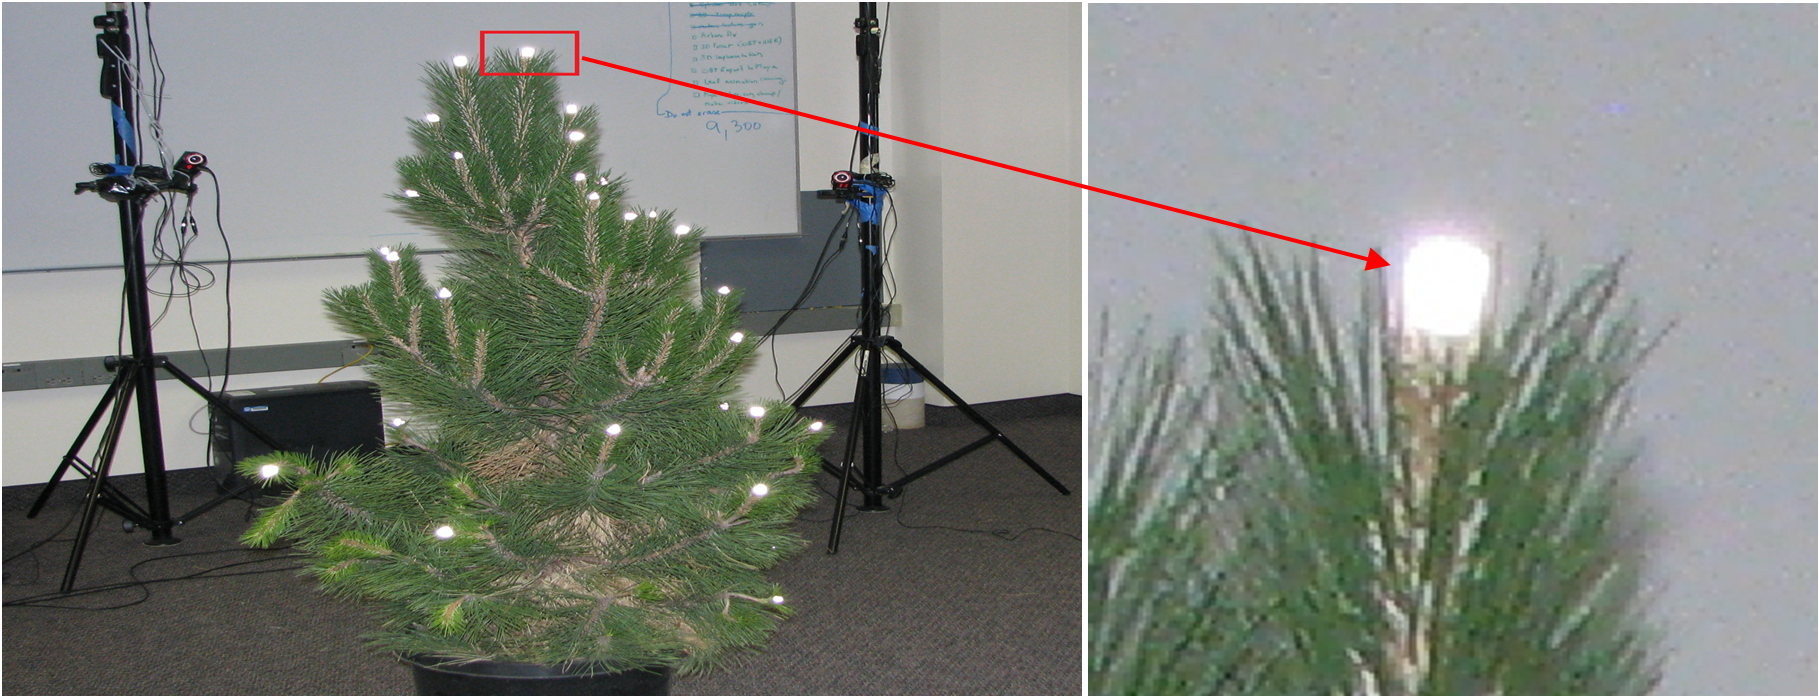
\includegraphics[width=5.0in]{Mocap}
\caption[Marker placement on the crown periphery.]{Marker placement on the crown periphery avoids occlusion while generating data that can be used to generate crown structure.}
\label{fig:mocap}
\end{figure}

Our design requires less user intervention, produces cleaner motion capture data , and may support animation of tree motion.

\section{Data Processing}
\label{sec:Dataprocessing}

Simply inferring positions from one frame of captured data is not adequate due to noise. These branch tips with markers are called "recorded" or "captured" tips. However, the initial locations of recorded branch tips may contain errors due to noise in either the system or the capture environment. 

A clustering algorithm approximates a single initial position from a collection of captured initial positions for recorded branch tips while minimizing error from the motion capture system. The clustering algorithm analyzes positions over many frames of motion capture data and eliminates gaps and noise. Gaps occur when a marker is not present in a frame. This algorithm uses forward differencing to predict a position for a marker at frame $M$ based on positions in previous frames. The closest marker in the next frame is added to the motion trace for the marker if there is a marker located close enough to the predicted position. If there is no marker position recorded close enough to the predicted position, that marker is marked with no data, i.e. a gap, for that frame. Gaps are repaired using interpolation over the motion path for a marker. If the number of marker positions recorded for a marker over time is less than $1/4$ of the total frames, that partial marker trace is marked as noise and eliminated.

If the capture process includes several hundred frames of data in which the tree is not moving, averaging branch tip positions over these frames results in precise estimates of initial positions. In most cases, the number of markers inferred from the clustering process matches the number of markers placed on the tree.

\section{Generating 3D Tree Shape}

Particle flow is a well-studied approach to generating 3D branching structure for trees \cite{Reeves83particlesystems,Runions07,palubicki:siggraph09,neubert:acmtg07}. We adapt the method to motion capture data. The 3D tree crown boundary inferred from motion capture data constrains the particle range and preserves the original 3D tree silhouette. We use a stack of bounding boxes or convex hulls to represent the crown boundary. Particles, either generated randomly in the boundary or locations of branch tips recorded by motion capture, are moving towards trunk nodes. Three forces---gravity, internal force, and external force---drive the particle flow process. The paths of the particle flow produce branching structure. By attaching leaves to the branching structure, we generate a 3D tree model that has similar appearance as the natural tree shape. 

We synthesize a trunk in the center of the crown shape, as shown in Figure \ref{fig:PineTrunk}. Figure \ref{fig:PineTrunksubfig1} shows a photograph of a pine tree with markers placed on its crown. Figure \ref{fig:PineTrunksubfig2} contains a bounding box of these marker locations and a straight vertical line representing trunk shape. The length of the line is scaled by the crown height of the bounding box. On this line segment, we generate about 10 trunk nodes. Random offsets to these nodes in the x and z direction are added as shown in Figure \ref{fig:PineTrunksubfig3}.

\begin{figure}
\centering
        \begin{subfigure}[b]{0.22\textwidth}
                \centering
                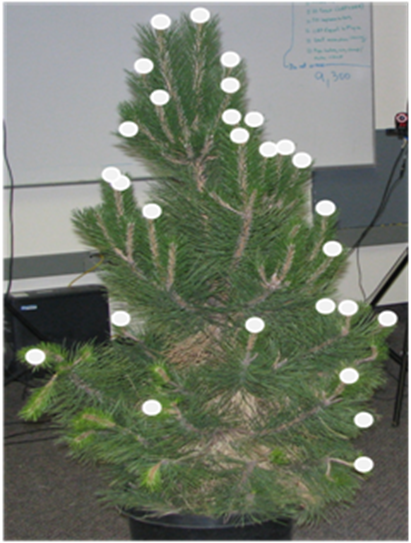
\includegraphics[width=\textwidth]{PineTrunk1}
                \caption{A pine tree with markers.}
                \label{fig:PineTrunksubfig1}
        \end{subfigure}
        ~
        \begin{subfigure}[b]{0.31\textwidth}
                \centering
                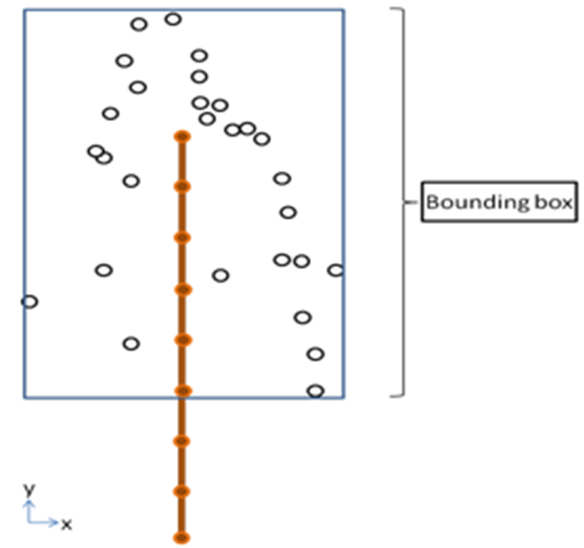
\includegraphics[width=\textwidth]{PineTrunk2}
                \caption{A straight line represents the trunk.}
                \label{fig:PineTrunksubfig2}
        \end{subfigure} 
        ~
        \begin{subfigure}[b]{0.30\textwidth}
                \centering
                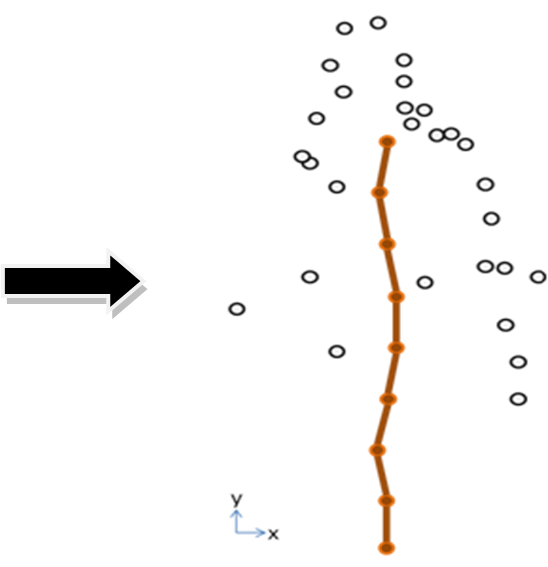
\includegraphics[width=\textwidth]{PineTrunk3}
                \caption{Adding random offsets looks more natural.}
                \label{fig:PineTrunksubfig3}
        \end{subfigure}             
\caption{A simple trunk model is added to the collection of branch tip positions.}
\label{fig:PineTrunk}
\end{figure}

A particle represents a branch tip. One group of particles is 3D positions of branch tips recorded from motion capture, which is described in Section \ref{sec:Dataprocessing}. Figure \ref{fig:PineTrunksubfig1} shows a photograph of a pine tree with markers placed on the crown. All the branch tip locations recorded by motion capture are labeled with white dots. These particles are shown in black circles in Figure \ref{fig:boundboxsubfig3} and Figure \ref{fig:ConvexHullPoints}. 

Because of motion capture's limited capability, we cannot record locations for every branch tip on the tree. Another group of particles is randomly generated within the bounded space of all the recorded branch tip positions. In Figure \ref{fig:boundboxsubfig3} and Figure \ref{fig:ConvexHullPoints}, these particles are green. 

Instead of using one single bounding box for the whole tree crown, we create a vertical stack of bounding boxes as shown in Figure \ref{fig:boundbox}. The new bounding boxes more closely match the tree shape. In Figure \ref{fig:boundboxsubfig3}, the crown height is evenly divided into four parts. Particles are randomly generated inside the smaller bounding boxes, as shown using green dots in Figure \ref{fig:boundboxsubfig3}. The total number of branch tips, including motion capture branch tips and randomly generated particles, is set to be similar to the original tree. The number of green dots in each box is proportional to the number of black dots. Therefore, we maintain a similar total amount and distribution of natural tree branch tips.

\begin{figure}
\centering
        \begin{subfigure}[b]{0.2\textwidth}
                \centering
                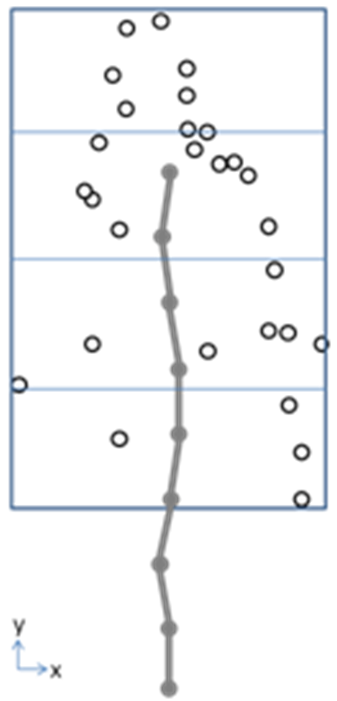
\includegraphics[width=\textwidth]{boundbox1}
                \caption{}
                \label{fig:boundboxsubfig1}
        \end{subfigure}
        ~
        \begin{subfigure}[b]{0.27\textwidth}
                \centering
                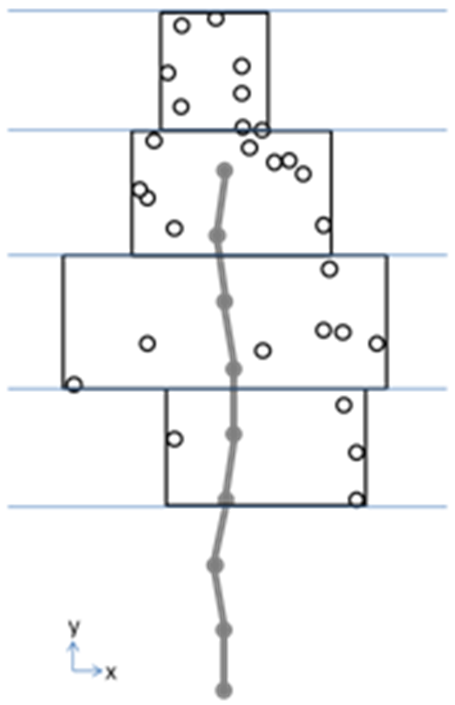
\includegraphics[width=\textwidth]{boundbox2}
                \caption{}
                \label{fig:boundboxsubfig2}
        \end{subfigure} 
        ~
        \begin{subfigure}[b]{0.2\textwidth}
                \centering
                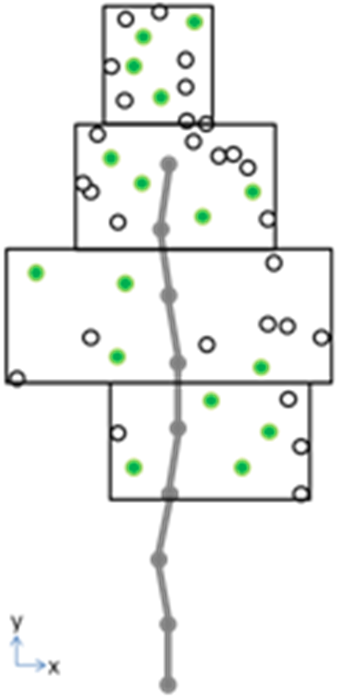
\includegraphics[width=\textwidth]{boundbox3}
                \caption{}
                \label{fig:boundboxsubfig3}
        \end{subfigure}             
\caption{New particles are added within a vertical stack of bounding boxes.}
\label{fig:boundbox}
\end{figure}

Alternatively, we use a convex hull for all the particles, as shown in Figure \ref{fig:ConvexHullPoints}. A convex hull provides more precise bounding space than the stack of bounding boxes. However, it requires a (slightly) more complex boundary detection scheme and more implementation details. Because of the precision that a convex hull brings, we recommend this approach for building a bounding volume.

\begin{figure}[!t]
\centering
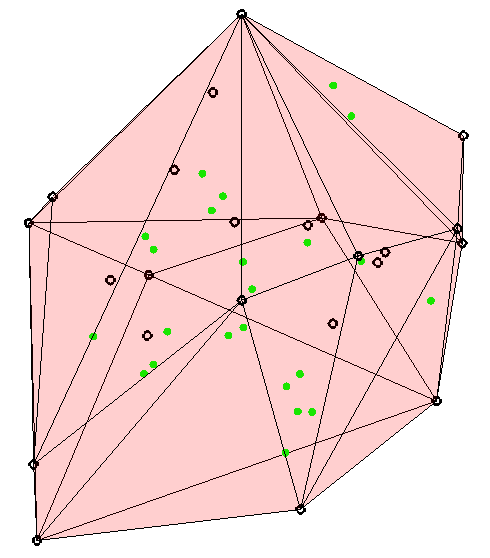
\includegraphics[scale=0.5]{ConvexHullPoints}
\caption[A convex hull for all the particles.]{A convex hull for all the particles. Particles in black color are from motion capture and particles in green color are randomly generated inside the convex hull.}
\label{fig:ConvexHullPoints}
\end{figure}

For the pine tree's trunk, we generate nine nodes in a straight vertical line and add random offsets in the x and z directions to these trunk nodes. The length of the line is scaled about 1.2 times the pine tree's crown height.

Trunk nodes contain a root attractor point and a nearest trunk point, as shown in Figure \ref{fig:flow}. The root attractor point, shown in green, is the trunk node closest to the lower bound of the bounding box for the entire crown. The nearest trunk point, which is shown in blue for the red particle in Figure \ref{fig:flowsubfig1}, is the closest trunk node to a single particle.

\begin{figure}
\centering
        \begin{subfigure}[b]{0.2\textwidth}
                \centering
                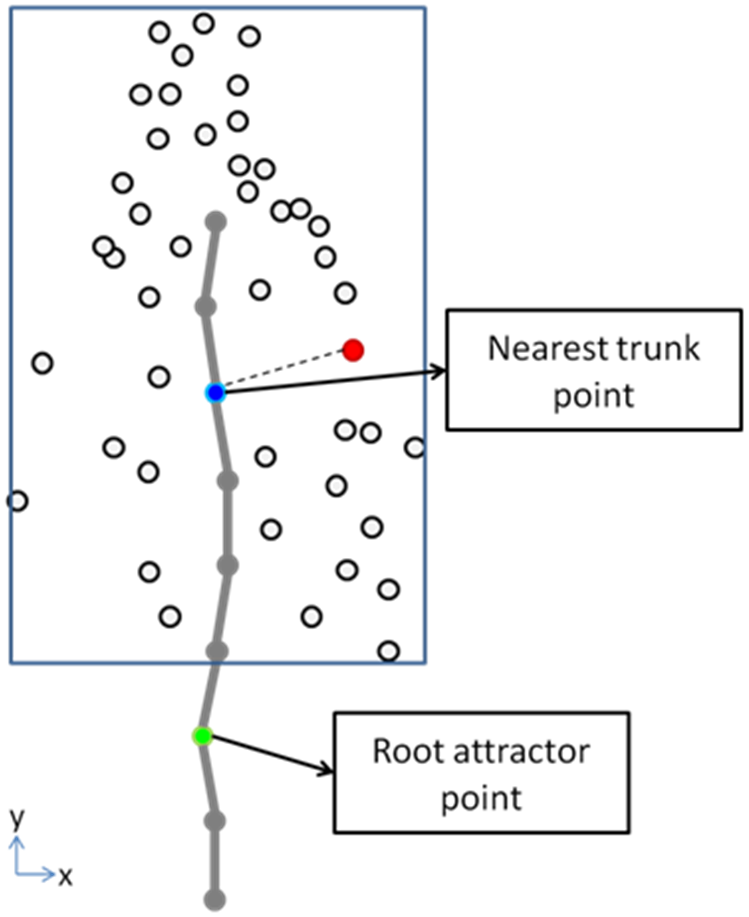
\includegraphics[width=\textwidth]{flow1}
                \caption{Flow direction depends on root attractor and nearest trunk point positions.}
                \label{fig:flowsubfig1}
        \end{subfigure}
        ~
        \begin{subfigure}[b]{0.3\textwidth}
                \centering
                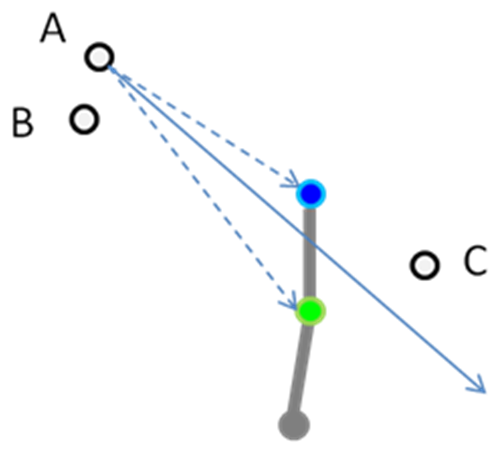
\includegraphics[width=\textwidth]{flow2}
                \caption{Root attractor point $S_r$ and nearest trunk point $S_t$.}
                \label{fig:flowsubfig2}
        \end{subfigure} 
        ~
        \begin{subfigure}[b]{0.3\textwidth}
                \centering
                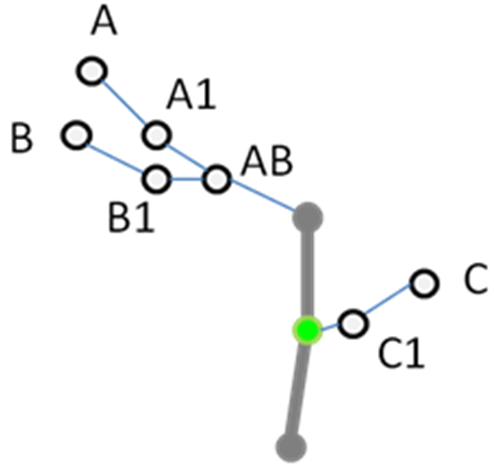
\includegraphics[width=\textwidth]{flow3}
                \caption{Particle flow ends when a particle merges with a neighbor or with the trunk.}
                \label{fig:flowsubfig3}
        \end{subfigure}             
\caption{A simple particle flow results in crown branching structure.}
\label{fig:flow}
\end{figure}

Particles move under directions of three forces: gravity, shape-format, and dominant wind. In Figure \ref{fig:forceTable}, we describe the direction and magnitude of each force. Gravity points vertically down to the ground. We assume that a particle has higher mass when it is closer to the trunk. This assumption follows the observation that when closer to the trunk, a branch has a larger radius. For a particle with higher mass, it has a larger magnitude of gravity and moves faster in the vertical downwards direction. Under this assumption, we set the magnitude of gravity proportional to the distance between a particle position $S_p$ and nearest trunk point $S_t$. 

We call the second force shape-format. Arborists distinguish styles of growth habit of trees using different classifications, such as excurrent and decurrent. The force tries to guide particle flow to follow the growth pattern of the original tree. Simulating different growth patterns requires different definitions of the shape-format force. In this research, we provide a simple example of shape-format definition. The shape-format force, shown in Figure \ref{fig:forceTable}, guides the particle flow process by height and depth of a tree crown. The direction of the force is pointing to the root attractor point $S_r$ from particle location $S_p$. The magnitude of the force is the average height of all the particles with a weight parameter $\alpha$. The higher the center of all the particles, the stronger the shape-format force points to the root attractor point $S_r$. This force is a pre-computed global force, which is a constant for all the particles. The direction of the force ensures that a particle finally merges to trunk nodes, and therefore all the branches grow towards the trunk.

The dominant wind direction is recorded from the motion capture setup, as described in Section \ref{sec:Motioncapturetrees}. Wind force is a special case of external force acting on the tree's branching shapes and structures. While doing motion capture, we record the location of the electrical fan. Because we only use one fan to create wind, that is the only source of explicit external force. Alternatively, the dominant wind direction can be inferred from tree movements recorded in motion capture data. Statistic methods, such as PCA , can estimate the dominate wind direction.

\begin{figure}[!t]
\centering
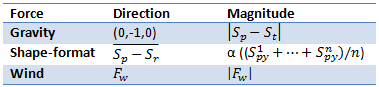
\includegraphics[scale=1.2]{forceTable}
\caption[Definition of three forces. ]{Forces: gravity, shape-format, and dominate wind. 
$S_p$: position of a particle. $S_{py}$ is position of a particle in $y$ direction.
$S_t$: position of the nearest trunk point.
$S_r$: position of the root attractor point.
$F_w$: wind measured from motion capture setup.
$\alpha$: scaling weight in range of [0, 1].
$n$: number of particles.
}
\label{fig:forceTable}
\end{figure}

The flow of particles starts at branch tips. Some particles merge in the flow process while others eventually reach and merge to the trunk. At each time step, we compute for step size and direction of a particle. The step size $L$ is:

\begin{equation}
\label{eqn:model1}
			L = \beta * ||S_p, S_t||,
\end{equation}

where $\beta$ is a tunable parameter in range of [0.1, 0.5] for most of our tree models. The step direction combines all the three forces. Figure \ref{fig:flowsubfig2} shows the computation of the direction for particle $i$, which is shown as particle $A$ in Figure \ref{fig:flowsubfig2}. Each force has a weighting parameter $\omega$ that tunes the relative importance of each vector and provides flexibility in creating branching shapes. The particle step direction $\vec{D_i}$ is given by

\begin{equation}
\label{eqn:model2}
	\vec{D_i} = (\omega_1*\vec{G_i} + \omega_2*\vec{S_i} + \omega_3*\vec{W_i} )/3,
\end{equation}

where $\omega$ is the weight of the direction, $\vec{G_i}$ is direction of gravity, $\vec{S_i}$ is direction of shape-format, and $\vec{W_i}$ is the wind direction for particle $i$ where $i\in[1,...,n]$.

Using step size $L$ and direction $\vec{D}$, the new particle position $V(m)$ is given by

\begin{equation}
\label{eqn:model3}
 V(m) = V(m-1) + L*\vec{D_i},
\end{equation}

where $m$ is current time step and $V(m-1)$ is the particle position at the last time step.

At each time step, after updating all the particle positions, particles might be merged. When the distance between a pair of particles is less than a predefined merging threshold, those particles are combined. When the distance between a particle and a trunk point falls below a predefined merging threshold, that particle is merged with the trunk. In Figure \ref{fig:flowsubfig3}, we demonstrate the paths of particle flow. Particle $A$, $B$, and $C$ are moved using the step and direction. Particle $A$ and $B$ are merged at point $AB$ and finally merged to the trunk. Particle $C$ merged to the trunk point after two time steps of movement.

\section{Adding Leaves}

Tree leaves are visually important to 3D tree models. After the branching structure is generated, leaves are attached. We use predefined leaf shapes, growth patterns, densities, and sizes. Also, because leaves do not always start growing at the beginning of a branch, we set a parameter called the leaf starting point. This parameter is proportional to a branch length. For example, when the parameter is $0.3$, it starts leaves after the point that is $0.3$ times the branch length away from the branch starting point. 

\section{Results}

Results are given for multiple trees, including maple and pine trees. The maple tree is instrumented with 24 markers placed on the periphery of the crown at branch tips and the pine tree is instrumented with 35 markers also located on branch tips. We collect the stationary locations of these markers for about 20 seconds at the capture rate of 100 frames/sec.

Figure \ref{fig:clustersubfig1} shows all the recorded locations as red dots for a single frame, and Figure \ref{fig:clustersubfig2} shows averaged locations from each cluster of marker positions for clusters in which the number of frames with a position in that cluster is $1/4$ of the total frame count. The data is recorded when the tree is stationary. Notice that a point in the blue box in Figure \ref{fig:clustersubfig1} is identified as noise and removed by the clustering algorithm. For the maple tree, after clustering and averaging only 24 markers remain and this matches the actual number of markers placed on the tree.

\begin{figure}
\centering
        \begin{subfigure}[b]{0.4\textwidth}
                \centering
                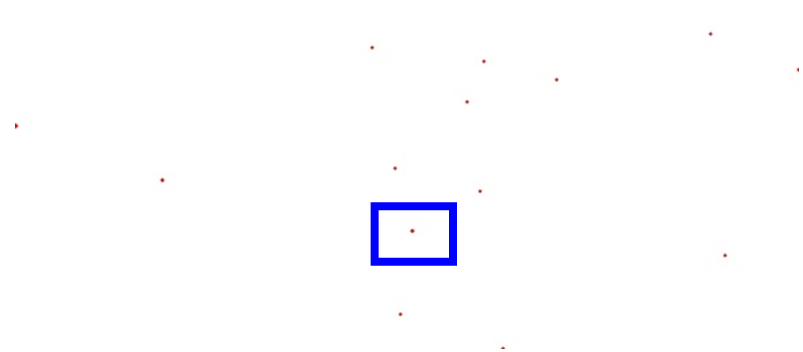
\includegraphics[width=\textwidth]{cluster1}
                \caption{Original collected data.}
                \label{fig:clustersubfig1}
        \end{subfigure}
        ~
        \begin{subfigure}[b]{0.4\textwidth}
                \centering
                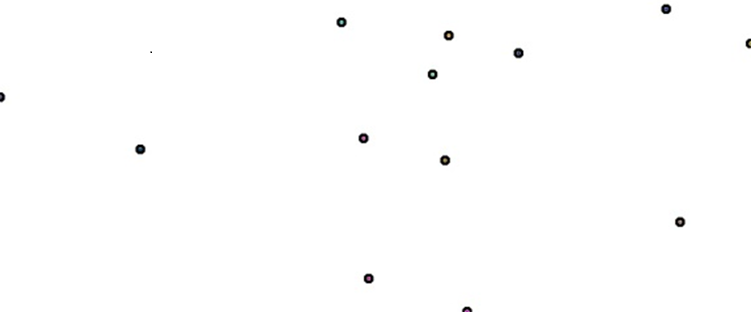
\includegraphics[width=\textwidth]{cluster2}
                \caption{Remaining branch tip locations after clustering.}
                \label{fig:clustersubfig2}
        \end{subfigure}     
        \caption{Clustering that removes noise that leads to spurious marker positions.}
        \label{fig:cluster}
\end{figure}

Although initial marker positions are collected before wind is applied when the tree is stationary, the data contain a small amount of noise, which can be removed to create a single initial marker position. In Figure \ref{fig:markerPath}, we show marker positions over time for two markers during the stationary phase. The horizontal axis shows time while the vertical axis shows a marker location in 3D space. In the first image, movement in each direction spans $10^{-3}$ meters. In addition, in the second image there is apparently a small periodic motion for the stationary branch tip. The range of motion is also within $10^{-3}$ meters. In both cases, averaging removes this small motion and estimates initial marker positions based on the average rather than a single position in a single frame.

\begin{figure}
\centering
        \begin{subfigure}[b]{0.42\textwidth}
                \centering
                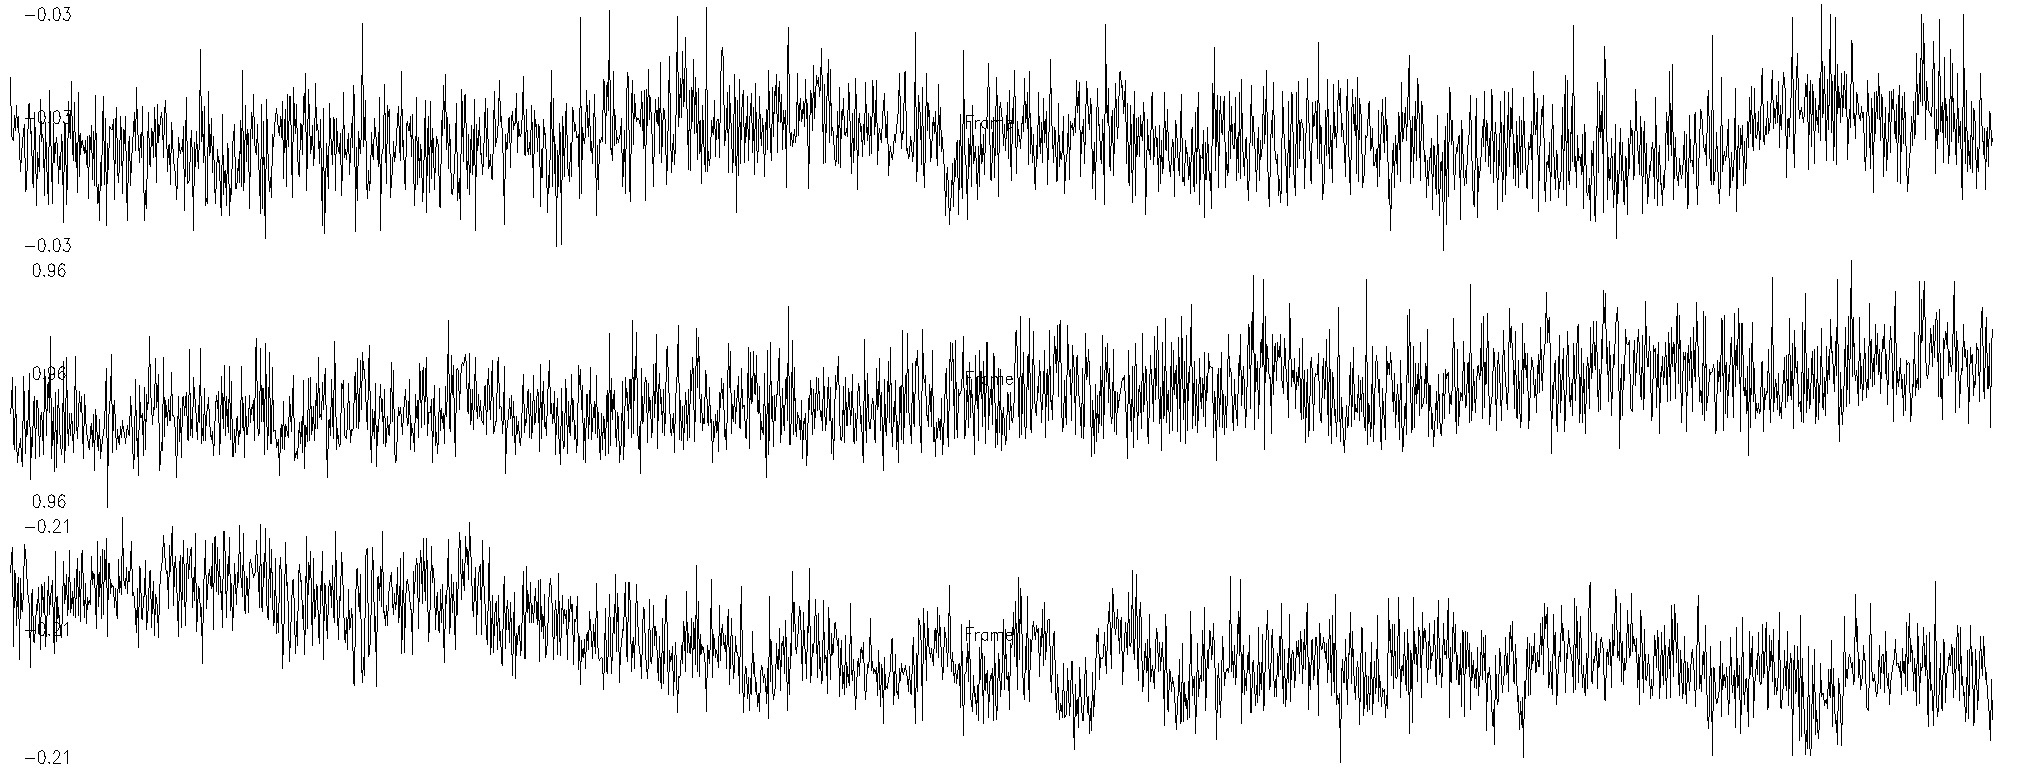
\includegraphics[width=\textwidth]{Marker0orig}
                \caption{Close to white noise.}
                \label{fig:markerPathsubfig1}
        \end{subfigure}
        ~
        \begin{subfigure}[b]{0.42\textwidth}
                \centering
                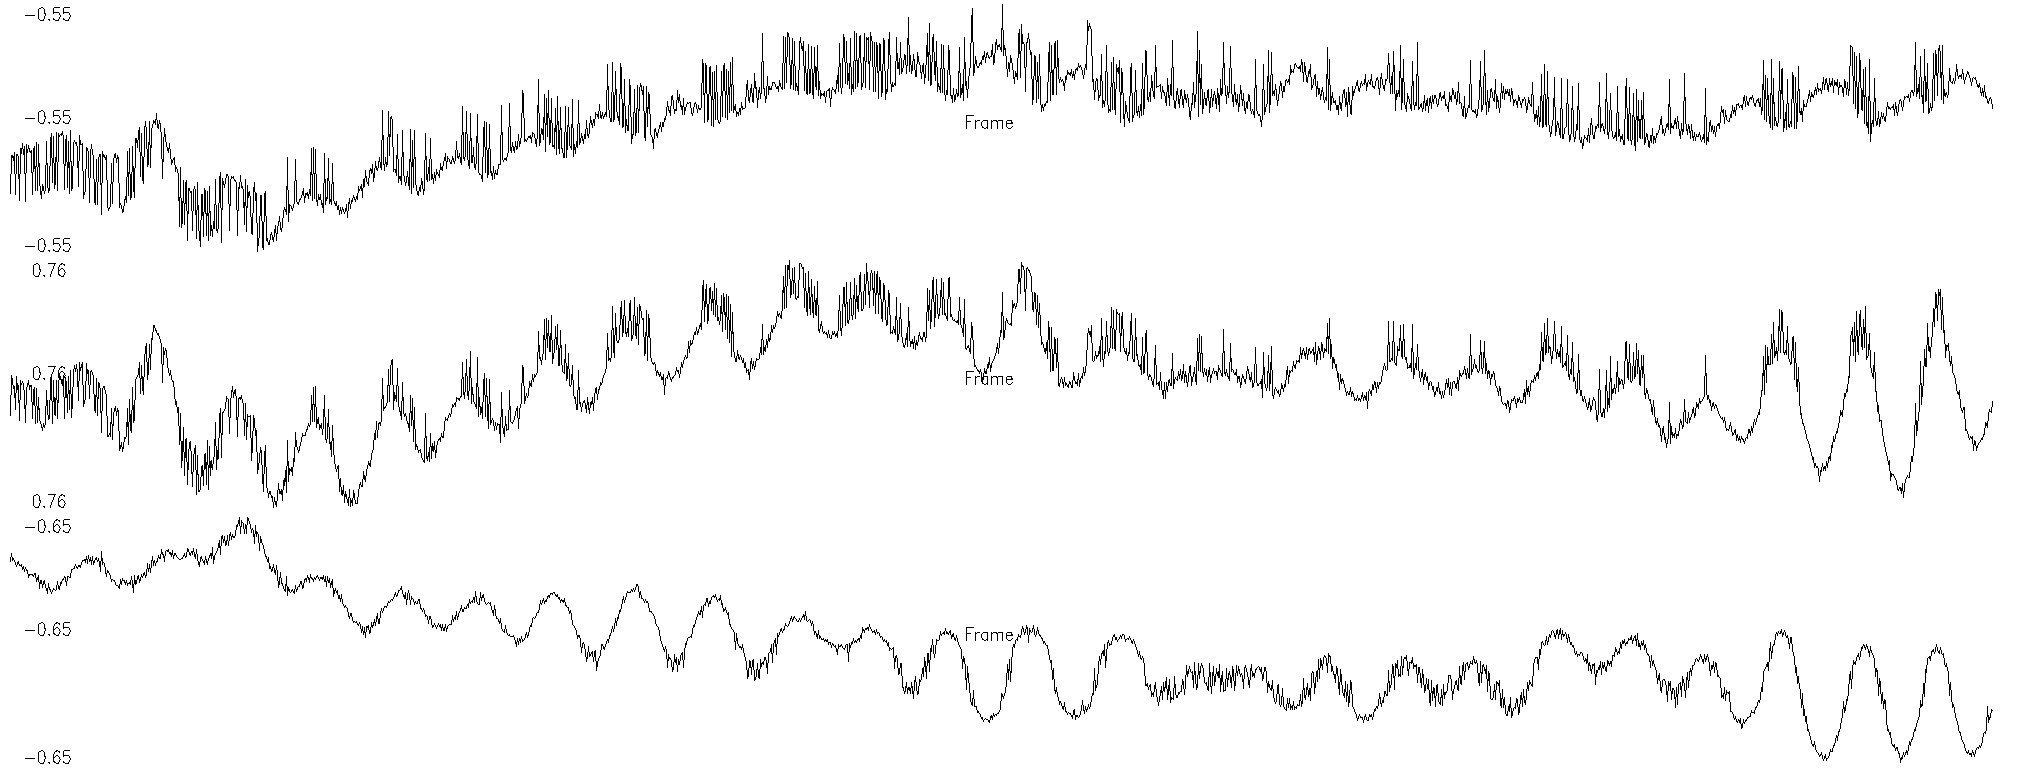
\includegraphics[width=\textwidth]{Marker5orig}
                \caption{Noise with apparent periods.}
                \label{fig:markerPathsubfig2}
        \end{subfigure}     
        \caption[Remove spurious motion. ]{Marker positions over time contain a small amount of spurious motion that is removed by averaging.}
        \label{fig:markerPath}
\end{figure}

A vertical stack of bounding boxes is a better approximation for the crown volume than a single bounding box and results in better crown shapes. Each bounding box contains branch tips and additional branch tips are added to each box. Figure \ref{fig:boundboxsizesubfig1} and Figure \ref{fig:boundboxsizesubfig2} illustrate the difference between tree crowns created with and without a stack of bounding boxes for a pine tree. Random particles placed uniformly within a single bounding box result in a cube shaped tree. Placing particles in a vertical stack of bounding boxes better approximates the original crown shape. Future work might include investigating non-uniform distributions of randomly inserted points instead of using bounding boxes. 

In Figure \ref{fig:boxTree} and Figure \ref{fig:convextTree}, we demonstrate the difference between tree shapes using stacked box bounding volumes and those using convex hull bounding volumes. The bounding box approach provides a looser bounding condition and allows more random factors in the final tree shape. The convex hull approach more closely approximates the original tree crown shape.

\begin{figure}
\centering
        \begin{subfigure}[b]{0.33\textwidth}
                \centering
                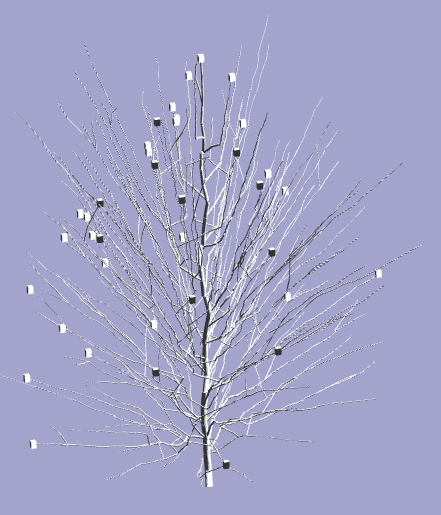
\includegraphics[width=\textwidth]{ResultBoundPine2}
                \caption{}
                \label{fig:boundboxsizesubfig1}
        \end{subfigure}
        ~
        \begin{subfigure}[b]{0.34\textwidth}
                \centering
                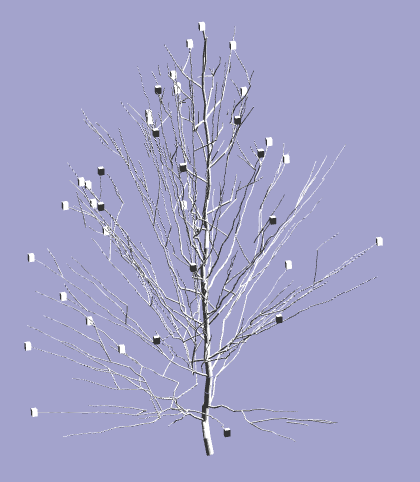
\includegraphics[width=\textwidth]{ResultBoundPine1}
                \caption{}
                \label{fig:boundboxsizesubfig2}
        \end{subfigure}
        ~
        \begin{subfigure}[b]{0.34\textwidth}
                \centering
                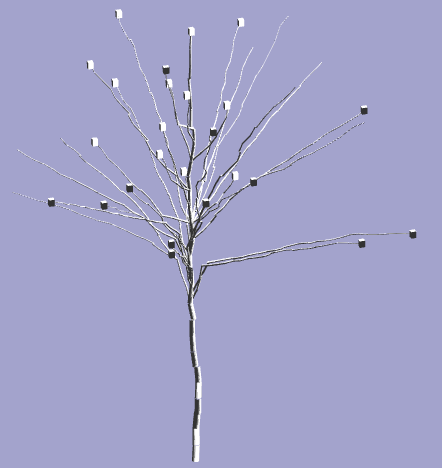
\includegraphics[width=\textwidth]{boundBoxTree}
                \caption{}
                \label{fig:boxTree}
        \end{subfigure}
        ~
        \begin{subfigure}[b]{0.33\textwidth}
				        \centering
				        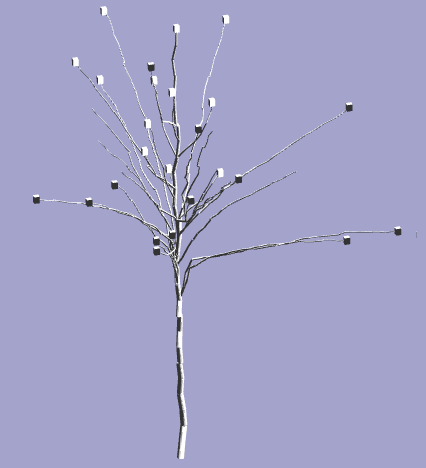
\includegraphics[width=\textwidth]{boundConvexTree}
				        \caption{}
				        \label{fig:convextTree}
        \end{subfigure}
\caption{Bounding volumes affect tree shape.}
\label{fig:boxConvex}
\end{figure}

Particle flow starting from branch tips and using our simplified algorithm results in tree crown shapes that mimic the shape of the tree from which data were collected. In the Figure \ref{fig:treemodelssubfig1}, we show the results from reconstructing a pine tree. 

\begin{figure*}[!t]
\centering
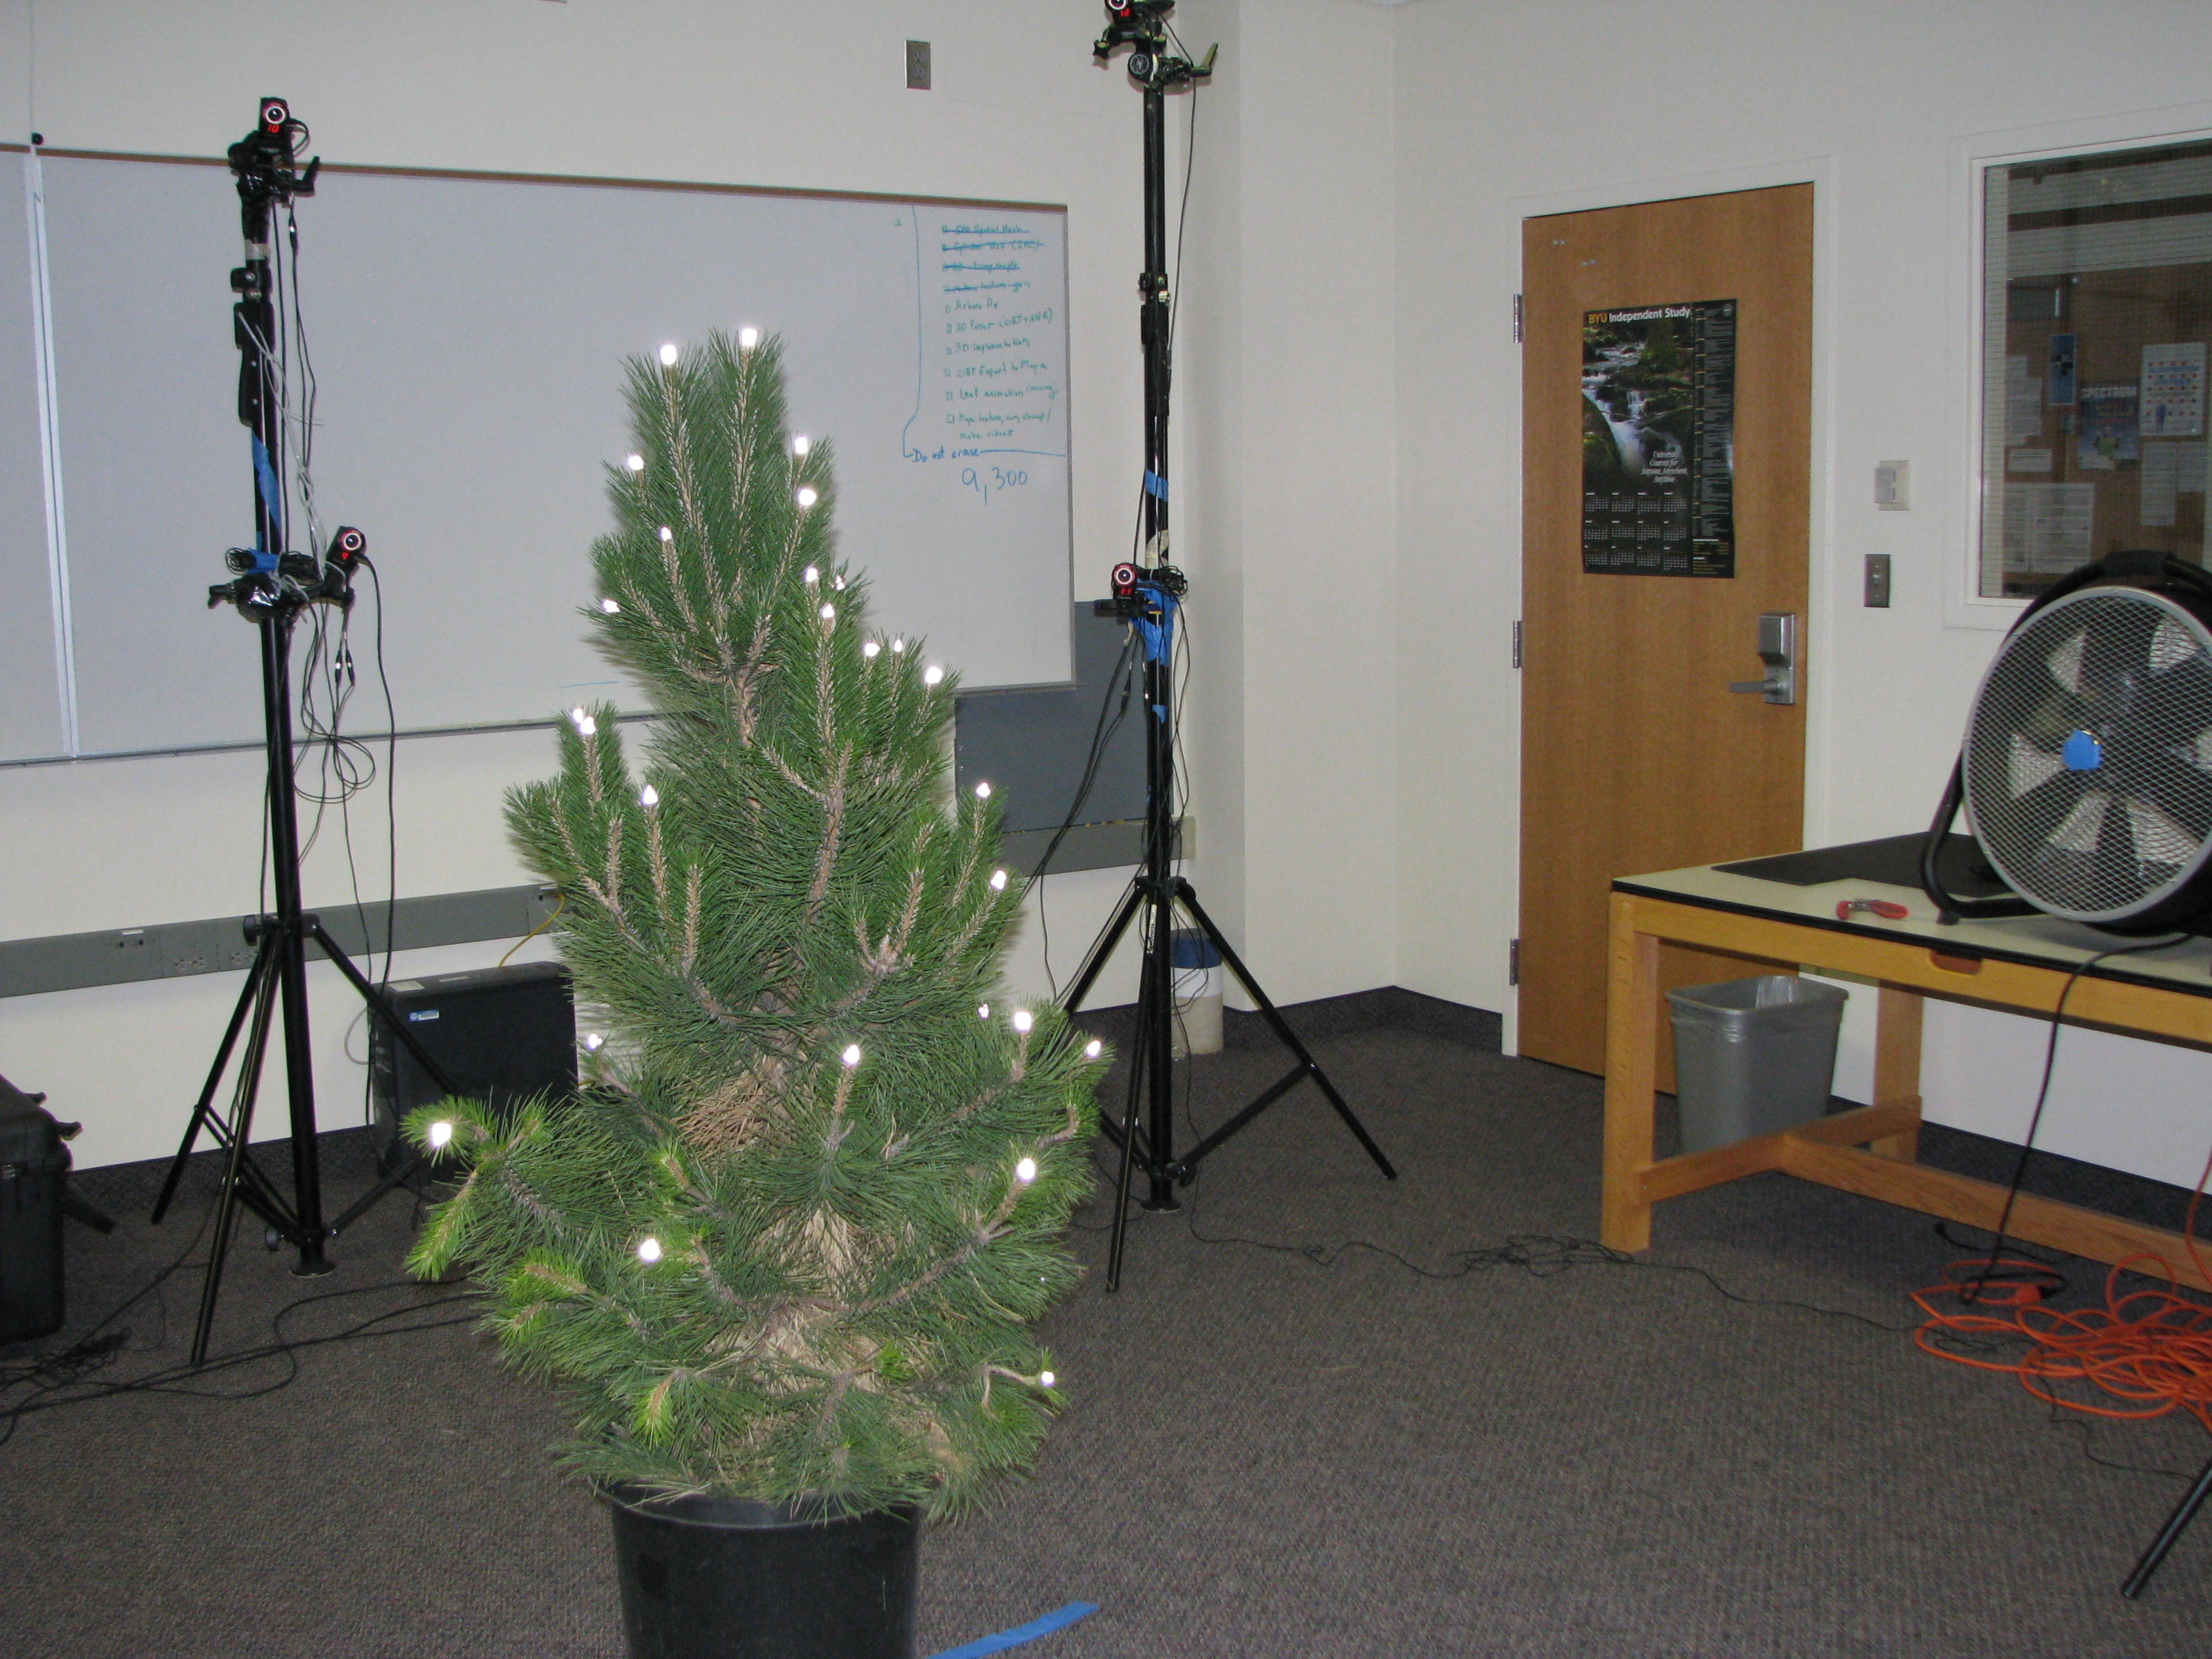
\includegraphics[scale=0.36]{Pine}
\caption[Pine tree model.]{Pine tree model. 3D tree models created from branch tip positions are similar to the shapes of the trees from which branch tip positions were collected.}
\label{fig:treemodelssubfig1}
\end{figure*}

Besides replaying the original tree shape, our approach has enough flexibility to produce different tree shapes based on the same set of motion capture data. Three forces with their scales create particles' moving paths, which represents branching structures. Figure \ref{fig:currency} demonstrates that shape-format force sets the global attracting trunk node, which controls the converging direction of particle flow. The resulting tree models display trees' growth styles in terms of excurrent and decurrent.

\begin{figure}
\centering
        \begin{subfigure}[b]{0.33\textwidth}
                \centering
                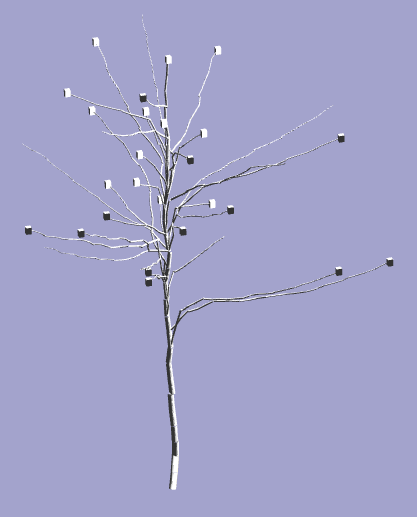
\includegraphics[width=\textwidth]{currency1}
                \caption{}
                \label{fig:currency1}
        \end{subfigure}
        ~
        \begin{subfigure}[b]{0.33\textwidth}
                \centering
                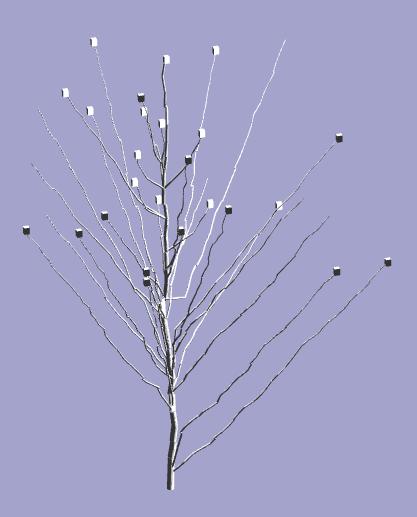
\includegraphics[width=\textwidth]{currency2}
                \caption{}
                \label{fig:currency2}
        \end{subfigure}
\caption{Shape-format force.}
\label{fig:currency}
\end{figure}

Figure \ref{fig:gravityTree} shows the impact of gravity on trees' shapes with various values for the weighting factor. When the factor is set to be negative, we create a special willow-like tree shape. 

\begin{figure}
\centering
        \begin{subfigure}[b]{0.3\textwidth}
                \centering
                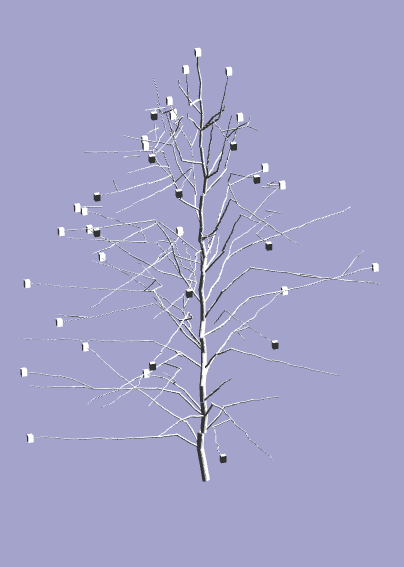
\includegraphics[width=\textwidth]{gravity001}
                \caption{weighting factor: 0.01}
                \label{fig:gravity001}
        \end{subfigure}
        ~
        \begin{subfigure}[b]{0.3\textwidth}
                \centering
                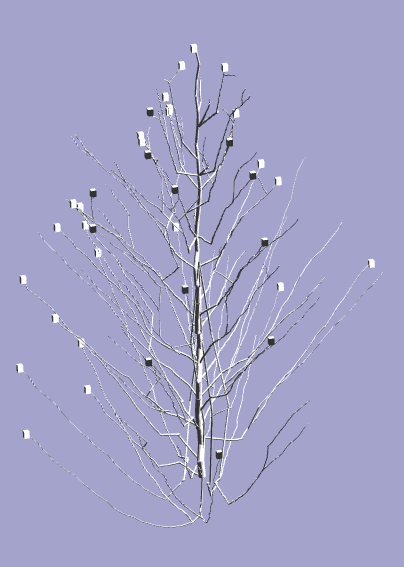
\includegraphics[width=\textwidth]{gravity020}
                \caption{weighting factor: 0.20}
                \label{fig:gravity020}
        \end{subfigure}
        ~
        \begin{subfigure}[b]{0.3\textwidth}
                \centering
                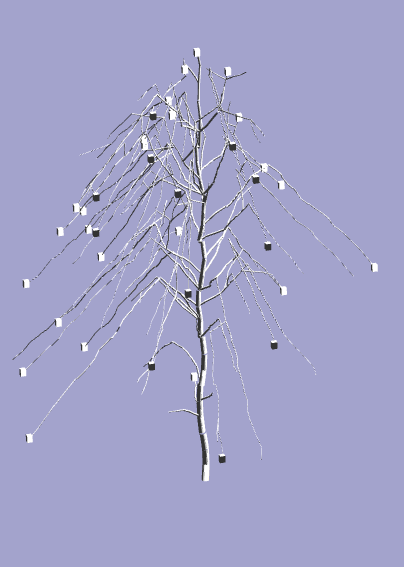
\includegraphics[width=\textwidth]{gravityNeg020}
                \caption{weighting factor: -0.20}
                \label{fig:gravityNeg020}
        \end{subfigure}
\caption{Tree shapes with different weight factors for gravity.}
\label{fig:gravityTree}
\end{figure}

Figure \ref{fig:windFactor} shows tree models with different weighting factors of wind force. Bigger values of the factor produces branches bending more toward the wind direction. Notice that the differences among these tree models are small, especially when compared to the influence from the other two forces. This is because the value of force for a global wind direction is set to be much smaller than that of the other two forces. Otherwise, when wind force dominates the direction of particle movement, the particles might not be able to merge to a tree's trunk and might violate natural tree's shape. 

\begin{figure}
\centering
        \begin{subfigure}[b]{0.3\textwidth}
                \centering
                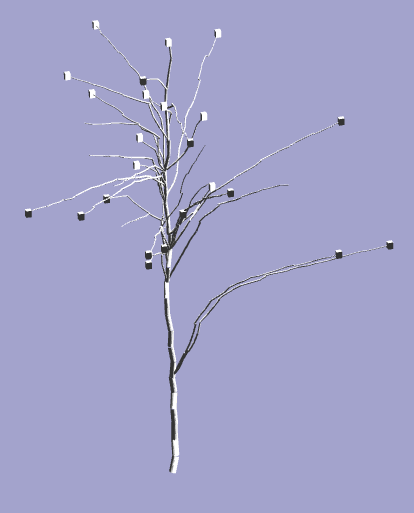
\includegraphics[width=\textwidth]{wind001}
                \caption{Weighting factor: 0.01.}
                \label{fig:wind001}
        \end{subfigure}
        ~
        \begin{subfigure}[b]{0.3\textwidth}
                \centering
                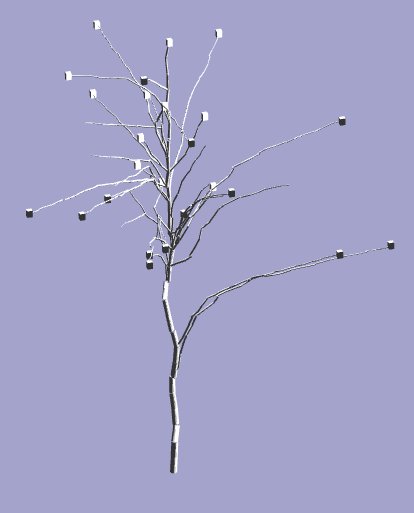
\includegraphics[width=\textwidth]{wind007}
                \caption{Weighting factor: 0.07.}
                \label{fig:wind007}
        \end{subfigure}
        ~
        \begin{subfigure}[b]{0.3\textwidth}
                \centering
                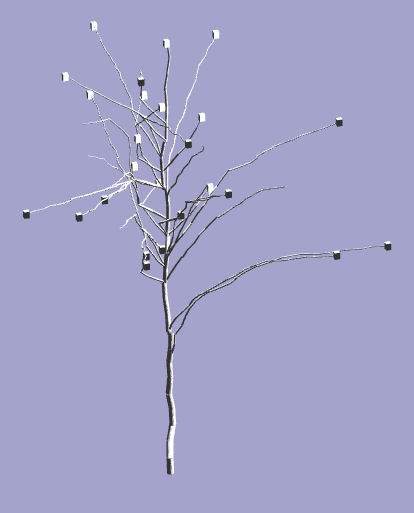
\includegraphics[width=\textwidth]{wind015}
                \caption{Weighting factor: 0.15.}
                \label{fig:wind015}
        \end{subfigure}
\caption{Tree shapes with different weighting factors for wind force.}
\label{fig:windFactor}
\end{figure}

In Figure \ref{fig:moreShapes}, we generate 3D tree models with different parameters for particle flow with the same set of motion capture data. These results demonstrate that our approach produces visually plausible tree shapes, which becomes scalable for more extended shapes through tweaking parameters of the three forces. 

\begin{figure}
\centering
        \begin{subfigure}[b]{0.3\textwidth}
                \centering
                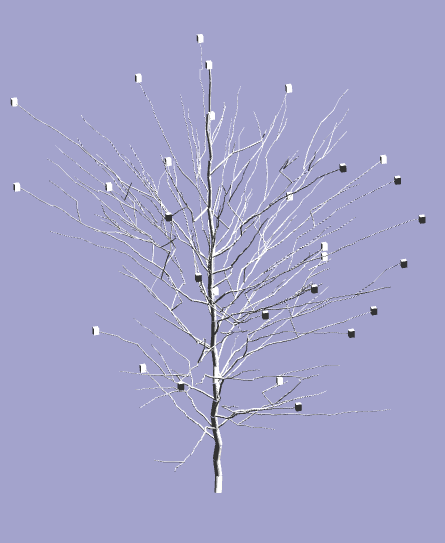
\includegraphics[width=\textwidth]{treediff1}
                \caption{}
                \label{fig:treediff1}
        \end{subfigure}
        ~
        \begin{subfigure}[b]{0.3\textwidth}
                \centering
                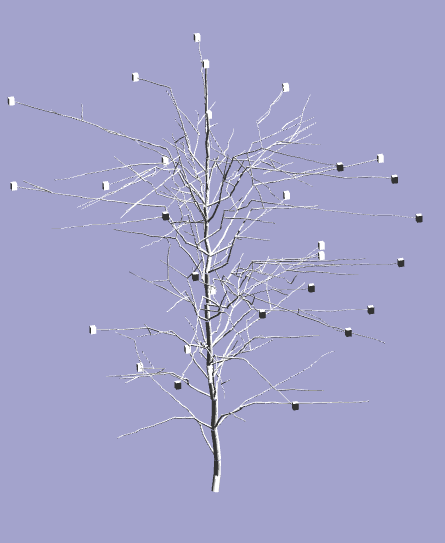
\includegraphics[width=\textwidth]{treediff2}
                \caption{}
                \label{fig:treediff2}
        \end{subfigure}
        ~
        \begin{subfigure}[b]{0.3\textwidth}
                \centering
                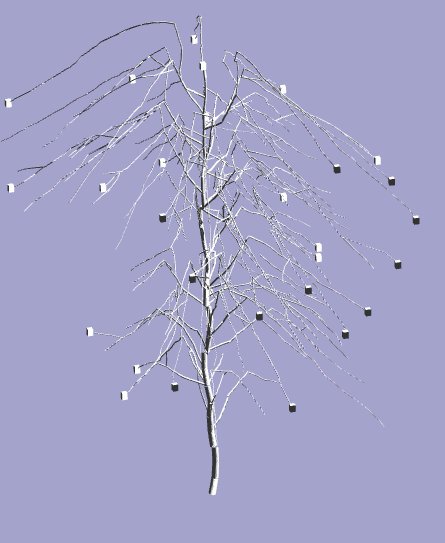
\includegraphics[width=\textwidth]{treediff3}
                \caption{}
                \label{fig:treediff3}
        \end{subfigure}
\caption{Various tree shapes.}
\label{fig:moreShapes}
\end{figure}

\section{Discussion and Future Work}

Placing retroreflective markers on branch tips evenly spaced throughout the crown on trees located in a passive optical motion capture arena results in data that can be used to reconstruct tree shape and which may be usable for replaying branch motion.  This can be done using a simplified particle flow system starting from recorded branch tip positions supplemented with additional random branch tip positions within a horizontal stack of bounding boxes and by setting two control parameters.  A new data collection process designed for trees may extend the use of motion capture to include trees and eventually other networks of non-rigid bodies. 

Future work includes extending the process to large trees outdoors as well as improving methods for animating the resulting tree models using the motion capture data.   We have reconstructed an approximate tree crown branching structure.  Replaying the captured motion data will require care to ensure that the motion of the approximate branching structure does not include uncorrelated motion for branch tips who share a common parent.